% Provenance (never printed): old premiere S material on the oceanic lithosphere
% (ophiolite-type layering, peridotite and gabbro, partial melting by decompression
% at the ridge, hydrothermalism, cooling and subsidence of the lithosphere with
% age); see sources/book2/PROVENANCE.md. Melting from figdata/grade-11/
% ridge_melting.py (adiabat and Hirschmann solidus), depth against age from
% depth_age.py (ETOPO1 and the Seton 2020 age grid). Partial melting is re-founded
% in Year 2 (mantle-melting); fault is Book 1's (g7), normal fault is defined here.
\chapter{Punggung Samudra dan Litosfer Samudra}\label{ch:g11:ocean-ridges}

Pada bulan Februari 1977 sebuah kereta luncur kamera yang ditarik 2500 meter di
bawah permukaan laut di atas Retakan Galápagos, di Pasifik timur, memotret lava
hitam yang gundul di punggung samudra itu, bingkai demi bingkai. Lalu
termometernya mencatat sedikit kenaikan suhu air, dan pada foto-fotonya lava itu
tertutup ratusan kerang putih. Beberapa hari kemudian kapal selam \emph{Alvin}
membawa dua ahli geologi turun ke tempat itu: air hangat yang berkilauan
mengalir keluar dari retakan-retakan lava, dan di sekitarnya hidup kerang
sepanjang lengan bawah, remis, dan kepiting putih; pada penyelaman berikutnya,
cacing tabung dengan ujung merah. Tidak ada yang menduga ada kehidupan di sana,
jadi tidak ada ahli biologi di kapal. Bab ini menjelaskan apa yang telah
ditemukan para ahli geologi itu: bagaimana dasar samudra dibuat di punggung
samudra, mengapa dasar itu panas di sana, dan apa yang terjadi padanya ketika ia
bergerak menjauh.
% ledger: whoi:alvin-1977

\begin{recall}
Di punggung samudra dasar samudra baru dibuat dan bergerak menjauh di kedua
sisi, sehingga umurnya bertambah seiring jaraknya dari sumbu; punggung-punggung
samudra membentuk sistem sepanjang sekitar \qty{65000}{km}, dengan lembah retakan
di sepanjang punggung yang lambat dan puncak yang mulus di sepanjang punggung yang
cepat (\cref{ch:g11:drift-to-spreading}). Lempeng-lempeng saling menjauh
melintasi punggung samudra dengan kecepatan beberapa sentimeter setahun, lebih
cepat melintasi Tinggian Pasifik Timur daripada melintasi Punggung Tengah
Atlantik (\cref{ch:g11:plate-motions}). \omterm{def:g11:lithosphere-asthenosphere:lithosphere}{Litosfer} adalah kulit luar yang kaku,
\omterm{def:g11:lithosphere-asthenosphere:lithosphere}{astenosfer} di bawahnya mengalir; suhu \omterm{def:g11:lithosphere-asthenosphere:lithosphere}{astenosfer} hanya naik sekitar
\qty{0.45}{\celsius} per kilometer kedalaman, dan suhu leleh batuan mantel naik
seiring kedalaman (\cref{ch:g11:lithosphere-asthenosphere}). Magma adalah
batuan cair di bawah permukaan, basalt adalah batuan gelap yang terbentuk dari
lava yang mendingin, dan sesar adalah rekahan yang di sepanjangnya batuan telah
bergeser (Buku 1, kelas 6 dan 7).
\end{recall}
% ledger: noaa:ridge, katsura10:adiabat, hirschmann:solidus

\section{Litosfer samudra}

Dua batuan yang jarang dijumpai di permukaan benua membentuk sebagian besar
\omterm{def:g11:ocean-ridges:oceanic-lithosphere}{litosfer samudra}.

\begin{definition}[Peridotit]\label{def:g11:ocean-ridges:peridotite}
Yang disebut \emph{peridotit}\index{peridotit} adalah batuan gelap berbutir kasar
yang sebagian besar terdiri atas mineral olivin, dengan sedikit piroksen.
Batuan ini biasanya hijau dan rapat. Sebagian besar mantel Bumi diyakini terdiri
atas peridotit.
\end{definition}

\begin{definition}[Gabro]\label{def:g11:ocean-ridges:gabbro}
Yang disebut \emph{gabro}\index{gabro} adalah batuan beku gelap berbutir kasar
yang terutama terdiri atas feldspar plagioklas dan piroksen. Komposisinya sama
dengan basalt, tetapi gabro mengkristal dengan lambat, jauh di bawah tanah,
sehingga kristal-kristalnya mempunyai waktu untuk tumbuh. Gabro adalah batuan
yang paling melimpah di \omterm{def:g11:ocean-ridges:oceanic-lithosphere}{kerak samudra} bagian dalam.
\end{definition}
% ledger: geo:peridotite, geo:gabbro

Mineral-mineral yang disebut di sini, yaitu olivin, piroksen, dan feldspar,
diperikan pada \cref{ch:g11:minerals}.

\begin{omfigure}
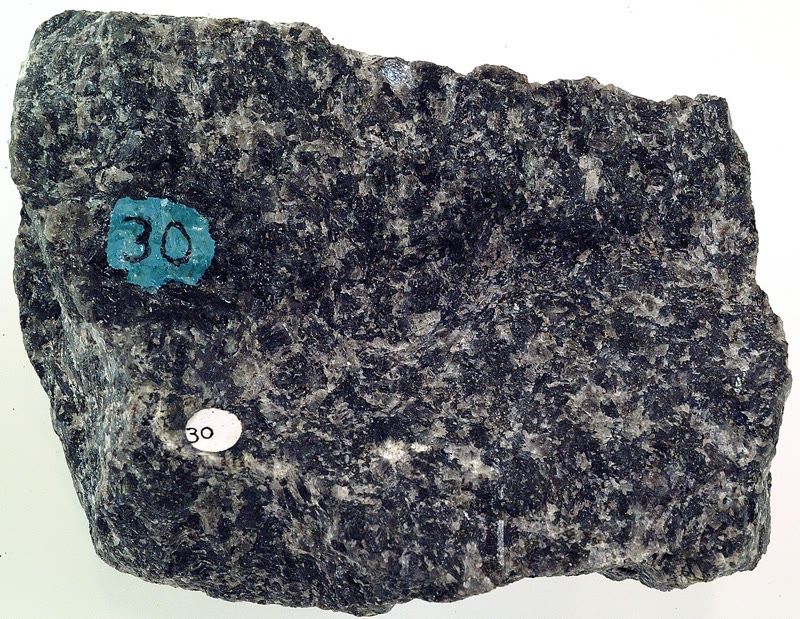
\includegraphics[height=4.2cm]{images/book2/g11-geodil-gabbro.jpg}\hspace{0.03\linewidth}%
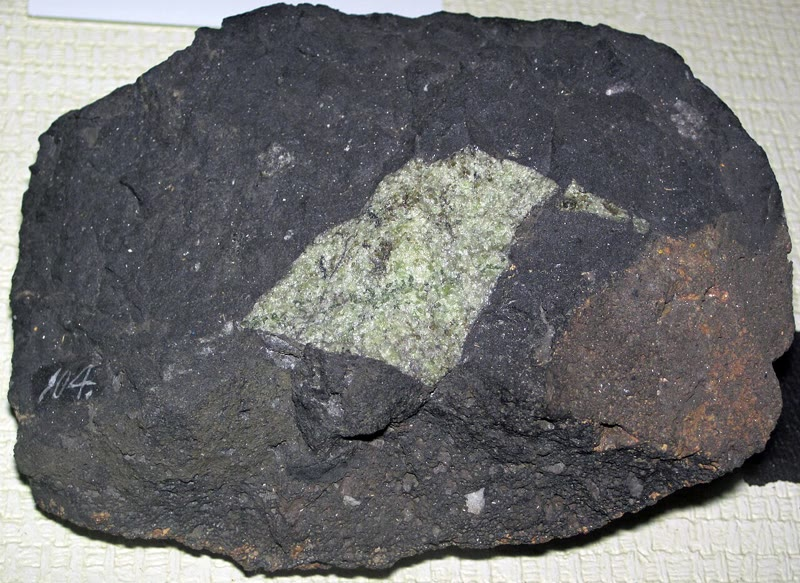
\includegraphics[height=4.2cm]{images/book2/g11-stjohn-peridotite.jpg}

{\small Kiri: \omterm{def:g11:ocean-ridges:gabbro}{gabro}, selebar \qty{9}{cm}, dengan kristal piroksen yang gelap dan
feldspar yang pucat, cukup besar untuk dilihat; foto Darla Sondrol (CC0).
Kanan: gumpalan \omterm{def:g11:ocean-ridges:peridotite}{peridotit} hijau dari mantel, yang terbawa naik di dalam lava
basalt hitam sebuah gunung api di Arizona; foto James St.~John (CC~BY~2.0).}
\end{omfigure}
% ledger: photo:g11-gabbro, photo:g11-peridotite

\begin{definition}[Kerak samudra; litosfer samudra]\label{def:g11:ocean-ridges:oceanic-lithosphere}
Yang disebut \emph{kerak samudra}\index{kerak samudra} adalah kerak dasar
samudra: basalt dan \omterm{def:g11:ocean-ridges:gabbro}{gabro} setebal sekitar \qty{7}{km}, yang dibuat di punggung
samudra. Yang disebut \emph{litosfer samudra}\index{litosfer samudra} adalah
kerak samudra bersama \omterm{def:g11:ocean-ridges:peridotite}{peridotit} kaku mantel paling atas di bawahnya.
\end{definition}

Survei seismik di seluruh samudra memberikan tebal rata-rata \omterm{def:g11:ocean-ridges:oceanic-lithosphere}{kerak samudra}
sebesar \qty{7.1}{km}, dengan selisih kira-kira \qty{0.8}{km}, jauh dari zona
rekahan dan titik panas. Lapisan-lapisannya diketahui dari pengeboran dalam dan
dari irisan dasar samudra tua yang terdorong naik ke atas benua. Pada tahun 2005
sebuah kapal bor menyelesaikan lubang sedalam \qty{1507}{m} ke dalam kerak
berumur 15 juta tahun di Pasifik timur, lubang pertama yang menembus dari lava,
melalui retas, sampai ke \omterm{def:g11:ocean-ridges:gabbro}{gabro}:
% ledger: white92:crust, iodp1256:section, geo:peridotite

\begin{itemize}
  \item di bagian atas, selimut tipis \emph{sedimen}, yang tidak ada di sumbu
        punggung dan lebih tebal di dasar yang lebih tua;
  \item \emph{lava basalt} setebal lebih dari \qty{800}{m}, yang meletus di
        dasar laut sebagai lembaran dan sebagai \emph{lava bantal}, tabung dan
        gumpalan lava yang membulat dengan kulit seperti kaca;
  \item \emph{retas berlapis}, setebal \qty{346}{m} di lubang ini: ratusan
        lembaran basalt yang tegak, masing-masing adalah retakan yang membeku
        tempat magma naik menuju letusan, berjajar seperti halaman-halaman buku;
  \item \emph{\omterm{def:g11:ocean-ridges:gabbro}{gabro}}, yang dicapai \qty{1407}{m} di bawah dasar laut, yaitu
        magma yang mengkristal dengan lambat di bawah retas, sampai ke \omterm{def:g11:seismic-structure:moho}{Moho};
  \item di bawah \omterm{def:g11:seismic-structure:moho}{Moho}, \emph{\omterm{def:g11:ocean-ridges:peridotite}{peridotit}} mantel.
\end{itemize}
% ledger: iodp1256:section, geo:basalt-ridges, geo:gabbro

\begin{omfigure}
\begin{tikzpicture}[x=1cm, y=-0.55cm, font=\footnotesize]
% to scale in depth: lavas 0.8 km, dykes 0.35 km (iodp1256:section), crust 7.1 km (white92:crust)
  \fill[omLithAlluv] (0,-0.25) rectangle (2.4,0);
  \fill[lith basalt] (0,0) rectangle (2.4,0.8);
  \fill[omLithBasalt!60] (0,0.8) rectangle (2.4,1.15);
  \foreach \x in {0.15,0.35,...,2.3} \draw[black!55, line width=0.3pt] (\x,0.8) -- (\x,1.15);
  \fill[lith gabbro] (0,1.15) rectangle (2.4,7.1);
  \fill[lith peridotite] (0,7.1) rectangle (2.4,9.0);
  \draw (0,-0.25) rectangle (2.4,9.0);
  \draw[line width=0.9pt] (0,7.1) -- (2.4,7.1);
  \foreach \d in {0,2,4,6,8} {\draw (-0.1,\d) -- (0,\d); \node[anchor=east] at (-0.1,\d) {\d};}
  \node[rotate=90, anchor=south] at (-0.75,4.5) {kedalaman di bawah dasar laut (\unit{km})};
  \draw[black!60] (2.4,-0.13) -- (2.7,-1.0) -- (2.85,-1.0);
  \node[anchor=west] at (2.85,-1.0) {sedimen};
  \draw[black!60] (2.4,0.4) -- (2.7,0.25) -- (2.85,0.25);
  \node[anchor=west] at (2.85,0.25) {lava: lava bantal dan aliran lembaran};
  \draw[black!60] (2.4,0.98) -- (2.7,1.6) -- (2.85,1.6);
  \node[anchor=west] at (2.85,1.6) {retas berlapis};
  \node[anchor=west] at (2.55,4.1) {gabro};
  \node[anchor=west] at (2.55,7.1) {Moho};
  \node[anchor=west] at (2.55,8.05) {peridotit mantel};
  \draw[decorate, decoration={brace, amplitude=5pt}] (7.9,0) -- (7.9,7.1)
    node[midway, right=7pt, align=left] {kerak samudra\\sekitar \qty{7}{km}};
\end{tikzpicture}

{\small Lapisan-lapisan \omterm{def:g11:ocean-ridges:oceanic-lithosphere}{kerak samudra}, dengan skala kedalaman yang sebenarnya.
Tebal lava dan retas adalah tebal di lubang dalam yang dibor di Pasifik timur;
tebal totalnya adalah rata-rata dari survei seismik. Selimut sedimen makin tebal
seiring umur dasar samudra.}
\end{omfigure}
% ledger: iodp1256:section, white92:crust

\begin{omfigure}
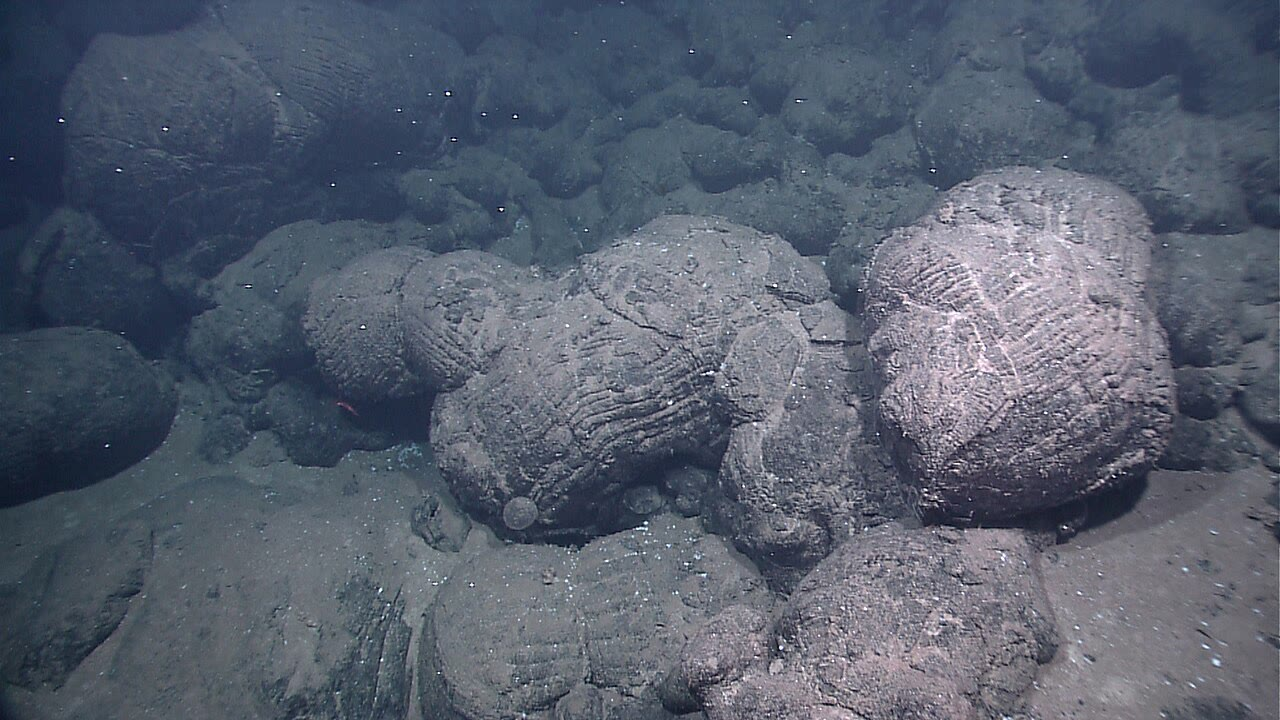
\includegraphics[width=0.8\linewidth]{images/book2/g11-noaa-pillow-lava.jpg}

{\small Lava bantal di Retakan Galápagos, pada kedalaman sekitar 2500 meter,
yang dipotret oleh kendaraan yang dikendalikan dari jauh pada tahun 2011. Setiap
bantal adalah lidah lava yang membeku dari luar begitu bertemu dengan air laut
yang dingin. Foto: NOAA Okeanos Explorer Program (domain publik).}
\end{omfigure}
% ledger: photo:g11-pillow-lava, whoi:alvin-1977 (depth of the rift floor)

\section{Meleleh tanpa dipanaskan}

Mantel di bawah punggung samudra adalah \omterm{def:g11:ocean-ridges:peridotite}{peridotit} padat, seperti di tempat lain.
Namun basalt dan \omterm{def:g11:ocean-ridges:gabbro}{gabro} setebal \qty{7}{km}, batuan cair yang membeku, berasal
darinya. Dari mana lelehan itu datang?

\begin{definition}[Pelelehan sebagian; pelelehan dekompresi]\label{def:g11:ocean-ridges:partial-melting}
Yang disebut \emph{pelelehan sebagian}\index{pelelehan sebagian} adalah
pelelehan sebagian saja dari suatu batuan: beberapa mineralnya, atau beberapa
komponennya, meleleh, sementara sisanya tetap padat.
Yang disebut \emph{pelelehan dekompresi}\index{pelelehan dekompresi} adalah
pelelehan sebagian batuan yang naik, sehingga makin lama makin kurang
termampatkan, tanpa dipanaskan.
\end{definition}

Ketika dua lempeng saling menjauh, \omterm{def:g11:lithosphere-asthenosphere:lithosphere}{astenosfer} naik di bawah punggung samudra
untuk mengisi celahnya. \omterm{def:g11:lithosphere-asthenosphere:lithosphere}{Astenosfer} naik terlalu cepat untuk kehilangan banyak
kalor, sehingga suhunya hanya turun sekitar \qty{0.45}{\celsius} per kilometer
selama naik. Suhu lelehnya, yang bergantung pada tekanan, turun jauh lebih cepat:
sekitar \qty{3.9}{\celsius} per kilometer pada kedalaman \qty{50}{km}. Pada
kedalaman tertentu batuan yang naik itu mencapai suhu lelehnya dan mulai
meleleh, meskipun tidak ada kalor yang ditambahkan.
% ledger: katsura10:adiabat, hirschmann:solidus, white92:crust; computed in
% figdata/grade-11/ridge_melting.py (solidus_slope_50km 3.89)

\begin{method}[Di mana mantel yang naik meleleh?]\label{met:g11:ocean-ridges:melting}
\begin{enumerate}
  \item Tuliskan suhu batuan yang naik pada setiap kedalaman: suhu
        potensialnya (suhu yang akan dimilikinya di permukaan)
        ditambah \qty{0.45}{\celsius} per kilometer kedalaman.
  \item Tuliskan suhu leleh batuan itu pada setiap kedalaman, dari
        tekanan pada kedalaman itu.
  \item Tentukan kedalaman tempat keduanya sama. Lebih dalam lagi, batuan itu
        padat; lebih dangkal, batuan itu sebagian cair.
\end{enumerate}
\end{method}

\begin{omfigure}
\begin{tikzpicture}
\begin{axis}[omrecord, omdepth, width=0.72\linewidth, height=6.4cm, xmin=1100, xmax=1700, ymin=0, ymax=150,
  xlabel={suhu (\unit{\celsius})}, ylabel={kedalaman (\unit{km})},
  xticklabel style={/pgf/number format/set thousands separator={}}, clip=true]
% computed in figdata/grade-11/ridge_melting.py; ledger: katsura10:adiabat, hirschmann:solidus, data:prem
\addplot[omProp, line width=1.0pt] table[x=solidus, y=z] {figdata/out/grade-11-ridge_melting-curves.dat};
\addplot[omDef, line width=1.0pt] table[x=ad1300, y=z] {figdata/out/grade-11-ridge_melting-curves.dat};
\addplot[omDef, densely dashed, line width=0.9pt] table[x=ad1400, y=z] {figdata/out/grade-11-ridge_melting-curves.dat};
\addplot[only marks, mark=*, mark size=1.8pt, black] coordinates {(1324.3,54.1) (1438.3,85.0)};
\node[font=\scriptsize, anchor=east, align=right] at (axis cs:1316,62) {pelelehan mulai,\\pada \qty{54}{km}};
\node[font=\scriptsize, anchor=east] at (axis cs:1432,89) {\qty{85}{km}};
\node[font=\scriptsize, text=omProp, anchor=west, align=left] at (axis cs:1560,40) {suhu\\leleh};
\node[font=\scriptsize, text=omDef, anchor=east, align=right] at (axis cs:1318,128) {mantel yang naik,\\$T_p = \qty{1300}{\celsius}$};
\node[font=\scriptsize, text=omDef, anchor=west, align=left] at (axis cs:1476,140) {$T_p = \qty{1400}{\celsius}$};
\end{axis}
\end{tikzpicture}

{\small Suhu batuan mantel yang naik di bawah punggung samudra (biru) dan suhu
lelehnya (jingga), terhadap kedalaman. Batuan dengan suhu potensial
\qty{1300}{\celsius} mulai meleleh pada kedalaman \qty{54}{km}; batuan yang
\qty{100}{\celsius} lebih panas (putus-putus) sudah meleleh pada \qty{85}{km}.
Suhu leleh \omterm{def:g11:ocean-ridges:peridotite}{peridotit} kering dari percobaan (Hirschmann, 2000).}
\end{omfigure}
% values: onset_1300_km 54.1, onset_1400_km 85.0, t_onset_1300 1324 (ridge_melting.py)

\begin{example}[Kedalaman pelelehan]\label{ex:g11:ocean-ridges:onset}
Untuk mantel dengan suhu potensial \qty{1300}{\celsius}, batuan yang naik
bersuhu $1300 + 0.45 \times 54 \approx \qty{1324}{\celsius}$ ketika mencapai
\qty{54}{km}, tepat suhu lelehnya pada kedalaman itu: pelelehan mulai pada
kedalaman sekitar \qty{54}{km}. Di atas kedalaman itu batuan terus meleleh
selama naik.
\end{example}

Hanya sebagian kecil \omterm{def:g11:ocean-ridges:peridotite}{peridotit} yang meleleh, dan lelehannya bukan \omterm{def:g11:ocean-ridges:peridotite}{peridotit}:
lelehan itu basalt. Lelehan basalt berkumpul dari seluruh daerah pelelehan, yang
membentang dari kedalaman awal pelelehan sampai dasar kerak; karena lebih ringan
daripada batuan padat di sekitarnya, lelehan itu naik ke sumbu punggung. Di sana
sebagian magma meletus sebagai lava, sebagian membeku sebagai retas di retakan
yang dilaluinya, dan sebagian mengkristal dengan lambat di bawahnya sebagai
\omterm{def:g11:ocean-ridges:gabbro}{gabro}. \omterm{def:g11:ocean-ridges:peridotite}{Peridotit} padat yang tertinggal, yang telah kehilangan basaltnya, menjadi
bagian mantel \omterm{def:g11:ocean-ridges:oceanic-lithosphere}{litosfer samudra}.
% ledger: asimow01:morb, geo:basalt-ridges, white92:crust

Di tempat punggung samudra melintasi wilayah mantel yang lebih panas, di sekitar
titik panas, pelelehan mulai lebih dalam, kolom batuan yang meleleh lebih
panjang, dan lebih banyak basalt yang dibuat: di sana kerak setebal sekitar
\qty{10}{km}, bukan 7. Sebaliknya, di bawah punggung yang sangat lambat, mantel
yang naik mempunyai waktu untuk kehilangan kalor, meleleh lebih sedikit, dan
membuat kerak yang luar biasa tipis.
% ledger: white92:crust

\begin{omfigure}
\begin{tikzpicture}[font=\footnotesize]
  % schematic section across a ridge axis, not to scale
  \fill[omSea!45] (-6,0) rectangle (6,1.2);
  \fill[lith basalt] (-6,0) -- (-0.25,0) -- (-0.25,-0.35) -- (-6,-0.6) -- cycle;
  \fill[lith basalt] (6,0) -- (0.25,0) -- (0.25,-0.35) -- (6,-0.6) -- cycle;
  \fill[lith gabbro] (-6,-0.6) -- (-0.25,-0.35) -- (-0.25,-1.4) -- (-6,-1.6) -- cycle;
  \fill[lith gabbro] (6,-0.6) -- (0.25,-0.35) -- (0.25,-1.4) -- (6,-1.6) -- cycle;
  \fill[lith basalt] (-0.3,0) rectangle (0.3,-0.35);
  \fill[lith gabbro] (-0.3,-0.35) rectangle (0.3,-1.45);
  \fill[omProp!70] (-0.8,-0.75) .. controls (-0.4,-0.55) and (0.4,-0.55) .. (0.8,-0.75)
     .. controls (0.4,-0.95) and (-0.4,-0.95) .. (-0.8,-0.75);
  \fill[omProp!70] (-0.12,0) rectangle (0.12,-0.62);
  \fill[lith peridotite] (-6,-1.6) -- (-0.25,-1.4) -- (0.25,-1.4) -- (6,-1.6) -- (6,-5) -- (-6,-5) -- cycle;
  % melting region
  \fill[omProp!35] (-3.2,-1.5) -- (0,-4.0) -- (3.2,-1.5) -- cycle;
  \node[align=center] at (0,-2.95) {daerah pelelehan};
  % isotherms deepening away from the axis
  \draw[omDef!70!black, densely dashed] (-6,-2.6) .. controls (-2.5,-2.0) and (-1,-1.1) .. (0,-1.0) .. controls (1,-1.1) and (2.5,-2.0) .. (6,-2.6);
  \draw[omDef!70!black, densely dashed] (-6,-4.2) .. controls (-3,-3.6) and (-1.2,-2.0) .. (0,-1.9) .. controls (1.2,-2.0) and (3,-3.6) .. (6,-4.2);
  \node[text=omDef!70!black, anchor=west] at (6.05,-2.6) {\qty{800}{\celsius}};
  \node[text=omDef!70!black, anchor=west] at (6.05,-4.2) {\qty{1200}{\celsius}};
  % flow arrows
  \draw[-{Stealth[length=5pt]}, line width=0.9pt] (0,-4.9) -- (0,-4.2);
  \draw[-{Stealth[length=5pt]}, line width=0.9pt] (-1.2,-4.8) .. controls (-1.0,-3.8) and (-2.2,-3.2) .. (-3.6,-3.2);
  \draw[-{Stealth[length=5pt]}, line width=0.9pt] (1.2,-4.8) .. controls (1.0,-3.8) and (2.2,-3.2) .. (3.6,-3.2);
  \draw[-{Stealth[length=5pt]}, line width=1.1pt] (-2,0.6) -- (-4,0.6);
  \draw[-{Stealth[length=5pt]}, line width=1.1pt] (2,0.6) -- (4,0.6);
  \node[anchor=south] at (-3,0.65) {lempeng};
  \node[anchor=south] at (3,0.65) {lempeng};
  \node[anchor=west] at (1.0,-0.8) {lensa magma};
  \node[anchor=east] at (-6.05,-0.3) {lava};
  \node[anchor=east] at (-6.05,-1.1) {gabro};
  \node[anchor=east] at (-6.05,-3.3) {mantel};
  \node[anchor=north] at (0,-5.05) {mantel naik dan meleleh};
\end{tikzpicture}

{\small Penampang melintang sumbu punggung samudra (gambar, tidak berskala).
Mantel naik di bawah sumbu dan meleleh sebagian; lelehan berkumpul dalam lensa
magma di bawah sumbu dan membangun kerak, yang dibawa lempeng-lempeng menjauh di
kedua sisi. Garis-garis suhu yang sama (putus-putus) terletak dekat dengan
permukaan di sumbu dan makin dalam makin jauh darinya: \omterm{def:g11:lithosphere-asthenosphere:lithosphere}{litosfer} menebal ketika
mendingin.}
\end{omfigure}

\section{Punggung yang cepat dan yang lambat}

Punggung-punggung samudra membuka dengan kecepatan yang sangat berbeda. Bila
dihitung dari kutub rotasi pada \cref{ch:g11:plate-motions}, Tinggian Pasifik
Timur pada \ang{30} LS membuka \qty{14.6}{cm} setahun, Punggung Tengah Atlantik
pada lintang yang sama \qty{3.3}{cm} setahun. Bentuk sumbunya tidak sama.
% ledger: nnr56:poles (computed in plate_velocities.py: epr30s_speed 145.8, atl30s_speed 32.7)

Di sepanjang punggung yang lambat, sumbunya berupa lembah sedalam 1 sampai
\qty{2}{km} dan selebar 20 sampai \qty{30}{km}. Magma yang mencapai sumbu terlalu
sedikit untuk mengisi celahnya terus-menerus: \omterm{def:g11:lithosphere-asthenosphere:lithosphere}{litosfer} yang dingin dan getas
tertarik terpisah dan patah di sepanjang sesar-sesar.

\begin{definition}[Sesar normal]\label{def:g11:ocean-ridges:normal-fault}
Yang disebut \emph{sesar normal}\index{sesar normal} adalah sesar miring yang di
sepanjangnya blok di atas bidang sesar telah bergerak turun relatif terhadap blok
di bawahnya. Sesar normal terbentuk di tempat kerak teregang.
\end{definition}

Lembah punggung yang lambat adalah blok yang telah turun di antara sesar-sesar
normal yang saling berhadapan; hampir semuanya miring ke arah sumbu. Blok yang
turun seperti itu di antara sesar-sesar normal disebut \emph{graben}.
% ledger: buck05:valley, usgs:normal-fault

Di sepanjang punggung yang cepat, magma cukup sering datang untuk mengisi
celahnya. Sumbunya berupa tinggian yang mulus dan landai, di atas lensa magma
yang terletak di bawahnya.
% ledger: buck05:valley, noaa:ridge

\begin{omfigure}
\begin{tikzpicture}[font=\footnotesize, x=0.24cm, y=0.9cm]
  % punggung lambat: lembah sumbu di antara sesar normal (tidak berskala, skala vertikal dibesarkan)
  \begin{scope}
    \fill[omSea!45] (-15,-0.7) rectangle (15,1.6);
    \fill[lith basalt] (-15,0.9) -- (-9,0.9) -- (-8.5,0.2) -- (-6,0.2) -- (-5.5,-0.6) -- (5.5,-0.6)
      -- (6,0.2) -- (8.5,0.2) -- (9,0.9) -- (15,0.9) -- (15,-2.2) -- (-15,-2.2) -- cycle;
    \draw[black!70] (-15,0.9) -- (-9,0.9) -- (-8.5,0.2) -- (-6,0.2) -- (-5.5,-0.6) -- (5.5,-0.6)
      -- (6,0.2) -- (8.5,0.2) -- (9,0.9) -- (15,0.9);
    \draw[fault] (-9,0.9) -- (-7.4,-2.2);
    \draw[fault] (-6,0.2) -- (-4.6,-2.2);
    \draw[fault] (9,0.9) -- (7.4,-2.2);
    \draw[fault] (6,0.2) -- (4.6,-2.2);
    % slip arrows on the hanging walls (the axis side of each fault): down along the fault
    \foreach \x/\y/\s in {-7.9/-0.5/1, -5.0/-1.3/1, 7.9/-0.5/-1, 5.0/-1.3/-1} {
      \draw[-{Stealth[length=3pt]}, omProp, line width=0.8pt] (\x+0.9*\s,\y+0.45) -- ++(0.3*\s,-0.6);
    }
    \draw[-{Stealth[length=5pt]}, line width=1pt] (-11,1.25) -- (-14,1.25);
    \draw[-{Stealth[length=5pt]}, line width=1pt] (11,1.25) -- (14,1.25);
    \node at (0,-0.25) {lembah sumbu};
    \node[anchor=north, align=center] at (0,-2.25) {punggung lambat: lembah\\di antara sesar normal};
  \end{scope}
  % fast ridge
  \begin{scope}[xshift=8.2cm]
    \fill[omSea!45] (-15,0) rectangle (15,1.6);
    \fill[lith basalt] (-15,0.3) .. controls (-6,0.4) and (-2,0.9) .. (0,0.95) .. controls (2,0.9) and (6,0.4) .. (15,0.3)
      -- (15,-2.2) -- (-15,-2.2) -- cycle;
    \fill[omProp!75] (-2.5,-0.9) .. controls (-1,-0.7) and (1,-0.7) .. (2.5,-0.9) .. controls (1,-1.1) and (-1,-1.1) .. (-2.5,-0.9);
    \draw[black!70] (-15,0.3) .. controls (-6,0.4) and (-2,0.9) .. (0,0.95) .. controls (2,0.9) and (6,0.4) .. (15,0.3);
    \node[anchor=north] at (0,-1.25) {lensa magma};
    \draw[-{Stealth[length=5pt]}, line width=1pt] (-8,1.25) -- (-14,1.25);
    \draw[-{Stealth[length=5pt]}, line width=1pt] (8,1.25) -- (14,1.25);
    \node at (0,1.3) {tinggian sumbu};
    \node[anchor=north, align=center] at (0,-2.25) {punggung cepat: tinggian landai\\di atas lensa magma};
  \end{scope}
\end{tikzpicture}

{\small Penampang melintang punggung yang lambat dan yang cepat (gambar, tidak
berskala; tingginya dibesarkan). Kiri: lembah sumbu punggung yang lambat, sedalam
1 sampai \qty{2}{km}, telah turun di antara sesar-sesar normal yang miring ke
arah sumbu (panah jingga: blok-blok di atas sesar meluncur turun). Kanan:
punggung yang cepat menjulang landai di atas lensa magma.}
\end{omfigure}
% ledger: buck05:valley

\begin{example}[Punggung yang lambat dan yang cepat]\label{ex:g11:ocean-ridges:rates}
Dalam sejuta tahun Tinggian Pasifik Timur pada \ang{30} LS membuat
$\qty{14.6}{cm/yr} \times 10^6\ \text{tahun} = \qty{146}{km}$ dasar samudra
baru, \qty{73}{km} di setiap sisi; Punggung Tengah Atlantik pada lintang yang
sama membuat \qty{33}{km}, \qty{16.5}{km} di setiap sisi. Lubang dalam di
Pasifik timur menembus kerak yang dibuat dengan laju lebih dari \qty{20}{cm}
setahun, salah satu pemekaran tercepat yang pernah tercatat.
\end{example}
% ledger: nnr56:poles (computed), iodp1256:section

\section{Ventilasi hidrotermal}

Kerak muda di sumbu itu panas, dan penuh retakan. Air laut menemukan jalan
masuk.

\begin{definition}[Sirkulasi hidrotermal; perokok hitam]\label{def:g11:ocean-ridges:hydrothermal}
Yang disebut \emph{sirkulasi hidrotermal}\index{sirkulasi hidrotermal} adalah
aliran air laut turun melalui retakan-retakan \omterm{def:g11:ocean-ridges:oceanic-lithosphere}{kerak samudra} yang panas, tempat
air itu dipanaskan oleh magma di bawahnya dan bereaksi dengan batuan, lalu naik
kembali ke dasar laut, tempat air itu keluar di \emph{ventilasi hidrotermal}.
Yang disebut \emph{perokok hitam}\index{perokok hitam} adalah ventilasi yang
mengeluarkan air yang sangat panas yang membawa logam-logam terlarut; ketika air
itu bertemu dengan air laut yang dingin, besi sulfida dan mineral-mineral lain
mengendap sebagai awan hitam, dan membangun cerobong di sekeliling ventilasi itu.
\end{definition}
% ledger: whoi:vents

Air \omterm{def:g11:ocean-ridges:hydrothermal}{perokok hitam} biasanya keluar dari cerobongnya pada suhu sekitar
\qty{350}{\celsius}, dan air ventilasi dapat mencapai \qty{400}{\celsius}. Air
itu tidak mendidih, karena dua setengah kilometer air menekannya. Cerobong-cerobong
itu dapat tumbuh lebih tinggi daripada \qty{10}{m}. Di sekitar ventilasi,
bakteri memperoleh energinya dari hidrogen sulfida dalam air ventilasi, dan
menjadi makanan bagi cacing tabung, udang, dan remis: kerang-kerang di Retakan
Galápagos hidup dari hal ini. Sebagian besar ventilasi terletak di sepanjang
punggung tengah samudra.
% ledger: whoi:vents, whoi:alvin-1977

\begin{omfigure}
\begin{minipage}[c]{0.6\linewidth}\centering
\begin{tikzpicture}[font=\scriptsize, x=0.8cm, y=0.62cm]
  \fill[omSea!45] (0,0) rectangle (10,3);
  \fill[lith basalt] (0,0) rectangle (10,-4);
  \fill[omProp!70] (2,-4.6) .. controls (4,-4.0) and (6,-4.0) .. (8,-4.6) -- (8,-5) -- (2,-5) -- cycle;
  \node at (5,-4.7) {magma};
  \fill[black!75] (4.7,0) -- (4.85,1.6) -- (5.15,1.6) -- (5.3,0) -- cycle;
  \fill[black!45, opacity=0.8] (5,1.7) circle (0.35) (5.2,2.2) circle (0.45) (4.9,2.7) circle (0.4);
  \draw[-{Stealth[length=4pt]}, omDef, line width=0.9pt] (1,0) .. controls (1,-2.5) and (2.5,-3.6) .. (4.2,-3.5);
  \draw[-{Stealth[length=4pt]}, omDef, line width=0.9pt] (9,0) .. controls (9,-2.5) and (7.5,-3.6) .. (5.8,-3.5);
  \draw[-{Stealth[length=4pt]}, omProp, line width=1.1pt] (5,-3.3) -- (5,-0.1);
  \node[align=center, text=omDef!80!black] at (1.6,1.0) {air laut\\dingin masuk};
  \node[align=left, anchor=west] at (5.6,1.4) {perokok hitam,\\sekitar \qty{350}{\celsius}};
  \node[align=left, anchor=west, text=omProp!80!black, fill=white, fill opacity=0.85, text opacity=1, inner sep=1.5pt] at (5.3,-1.8) {dipanaskan,\\naik};
\end{tikzpicture}
\end{minipage}\hfill
\begin{minipage}[c]{0.3\linewidth}\centering
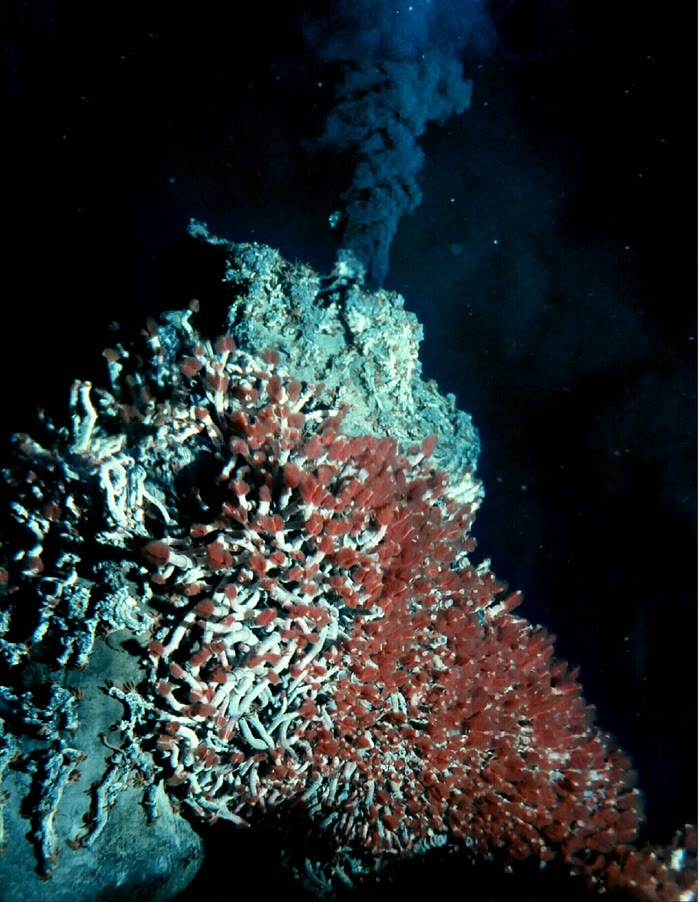
\includegraphics[width=\linewidth]{images/book2/g11-noaa-black-smoker.jpg}
\end{minipage}

{\small Kiri: \omterm{def:g11:ocean-ridges:hydrothermal}{sirkulasi hidrotermal} di sumbu punggung samudra (gambar, tidak
berskala). Kanan: \omterm{def:g11:ocean-ridges:hydrothermal}{perokok hitam} di Punggung Juan de Fuca, cerobongnya tertutup
cacing tabung berinsang merah; foto Universitas Washington dan NOAA
(domain publik).}
\end{omfigure}
% ledger: whoi:vents, photo:g11-black-smoker

\begin{history}[\emph{Alvin} di Retakan Galápagos, 1977]
Ekspedisi itu, yang dibiayai oleh Yayasan Sains Nasional Amerika Serikat, dimulai pada
8~Februari 1977 di atas kapal riset \emph{Knorr}. Kereta luncur kamera ANGUS,
yang ditarik \qty{2500}{m} di bawah permukaan laut di atas retakan itu, mencatat
kenaikan suhu air, dan pada bingkai-bingkai yang sama foto-fotonya menunjukkan
ratusan kerang putih dan cangkang remis cokelat di atas lava. Pada penyelaman
\emph{Alvin} yang ke-713, ahli geologi Jack Corliss dan Tjeerd van Andel
menemukan air bersuhu \qty{8}{\celsius} yang berkilauan keluar dari
retakan-retakan, lalu sampai \qty{17}{\celsius}, sedangkan air dalam di
sekitarnya bersuhu \qty{2}{\celsius}; kerang putih sepanjang sampai \qty{30}{cm}
menutupi daerah selebar sekitar \qty{50}{m}. Tidak ada ahli biologi di kapal:
ekspedisi itu datang untuk mencari air panas, dan menemukan komunitas hewan yang
tidak pernah dibayangkan siapa pun.
\end{history}
% ledger: whoi:alvin-1977

\section{Mendingin, menebal, tenggelam}

Ketika bergerak menjauhi sumbu, \omterm{def:g11:lithosphere-asthenosphere:lithosphere}{litosfer} mendingin dari atas, melalui samudra
dingin di atasnya. Lapisan yang telah mendingin makin tebal seiring waktu:
\omterm{def:g11:lithosphere-asthenosphere:lithosphere}{litosfer} menebal, dari beberapa kilometer di sumbu sampai sekitar seratus
kilometer di dasar yang tua. Batuan yang mendingin menyusut dan menjadi lebih
rapat, sehingga \omterm{def:g11:lithosphere-asthenosphere:lithosphere}{litosfer} mengapung lebih rendah di atas \omterm{def:g11:lithosphere-asthenosphere:lithosphere}{astenosfer} (\omterm{def:g11:lithosphere-asthenosphere:isostasy}{isostasi},
\cref{ch:g11:lithosphere-asthenosphere}): dasar samudra tenggelam seiring
umurnya. Untuk benda yang mendingin secara konduksi dari permukaannya, tebal
lapisan yang telah mendingin bertambah sebanding dengan akar kuadrat waktu.
% ledger: ps77:depth-age, rs09:lab

\begin{proposition}[Kedalaman dasar samudra terhadap umurnya]\label{prop:g11:ocean-ridges:depth-age}
Rata-rata, dasar samudra berumur $t$ (dalam juta tahun) terletak pada kedalaman
\[
  d(t) = 2500 + 350\sqrt{t} \quad \text{meter} \qquad (0 \le t \le 70),
\]
dan, untuk dasar yang lebih tua daripada sekitar 20 juta tahun,
\[
  d(t) = 6400 - 3200\,e^{-t/62.8} \quad \text{meter}:
\]
dasar itu tenggelam dengan cepat selama masih muda, lalu makin lama makin lambat,
menuju sekitar \qty{6400}{m}. (Diterima tanpa bukti: rumus-rumus itu dicocokkan
dengan kedalaman Pasifik Utara dan Atlantik Utara, yang dikoreksi untuk berat
sedimennya, oleh Parsons dan Sclater pada tahun 1977.)
\end{proposition}
% ledger: ps77:depth-age

Akar kuadrat membuat dasar yang muda tenggelam dengan cepat: dalam sejuta tahun
pertamanya dasar itu tenggelam \qty{350}{m}, dalam tiga juta tahun berikutnya
\qty{350}{m} lagi, dan antara 16 dan 64 juta tahun \qty{1400}{m}, sama banyaknya
dengan enam belas juta tahun pertamanya. Hukum eksponensial memerikan bagaimana
dasar yang tua berhenti tenggelam: dasar itu berperilaku seakan-akan lempeng yang
mendingin itu mempunyai tebal yang tetap, sekitar \qty{125}{km}.
% ledger: ps77:depth-age

\begin{omfigure}
\begin{tikzpicture}
\begin{axis}[omrecord, omdepth, width=0.82\linewidth, height=6.2cm, xmin=0, xmax=180, ymin=2000, ymax=6600,
  xlabel={umur dasar samudra (juta tahun)}, ylabel={kedalaman (\unit{m})},
  yticklabel style={/pgf/number format/set thousands separator={}},
  legend style={font=\scriptsize, at={(0.5,-0.32)}, anchor=north, legend columns=3, /tikz/every even column/.append style={column sep=6pt}}, legend cell align=left]
% computed in figdata/grade-11/depth_age.py; ledger: data:etopo1, data:b2-seafloor-age, ps77:depth-age
\addplot[only marks, mark=*, mark size=1.3pt, black!70, error bars/.cd, y dir=both, y explicit]
  table[x=age, y=depth, y error minus=em, y error plus=ep] {figdata/out/grade-11-depth_age-bins.dat};
\addplot[omProp, line width=1.0pt] table[x=age, y=depth] {figdata/out/grade-11-depth_age-sqrt.dat};
\addplot[omDef, line width=1.0pt, densely dashed] table[x=age, y=depth] {figdata/out/grade-11-depth_age-exp.dat};
\legend{{terukur: median dan separuh tengah}, {$2500 + 350\sqrt{t}$}, {$6400 - 3200\,e^{-t/62.8}$}}
\end{axis}
\end{tikzpicture}

{\small Kedalaman dasar samudra terhadap umurnya: untuk setiap pita umur selebar
5 juta tahun, median kedalaman semua sel satu derajat di samudra-samudra dunia,
dan rentang separuh tengahnya. Dasar yang muda mengikuti hukum akar kuadrat dengan
dekat; dasar yang lebih tua terletak lebih dangkal daripada hukum-hukum itu,
karena sel-selnya mencakup sedimen dan gunung api. Data: ETOPO1 (NOAA) dan umur
dasar samudra menurut Seton dan kawan-kawan (2020); hukum Parsons dan Sclater
(1977).}
\end{omfigure}
% values (depth_age.py): median 2.5-5 Myr 3114 (law 3178), 60-65 Myr 4648 (law 5267), fit a 2727 b 255

Kedalaman terukur dasar yang muda sesuai dengan hukum itu sampai sekitar
\qty{100}{m}. Pada dasar yang lebih tua, median yang terukur terletak beberapa
ratus meter di atas hukum-hukum itu. Hukum-hukum itu memerikan kedalaman dasar itu
sendiri, seakan-akan sedimennya disingkirkan; sel-sel yang terukur masih membawa
sedimennya, yang makin tebal seiring umur dasar dan setebal lebih dari satu
kilometer di dasar yang paling tua di Atlantik Utara bagian barat, dan sel-sel itu
mencakup gunung bawah laut dan dataran tinggi vulkanik.
% ledger: ps77:depth-age; values from depth_age.py

Karena itu \omterm{def:g11:ocean-ridges:oceanic-lithosphere}{litosfer samudra} yang tua tebal, dingin, dan rapat. Bab berikutnya
menunjukkan bahwa \omterm{def:g11:lithosphere-asthenosphere:lithosphere}{litosfer} itu dapat menjadi lebih rapat daripada \omterm{def:g11:lithosphere-asthenosphere:lithosphere}{astenosfer} di
bawahnya, dan tenggelam kembali ke dalam mantel (\cref{ch:g11:subduction-zones}).

\section{Latihan}

\begin{exercise}[$\star$]\label{exo:g11:ocean-ridges:1}
Definisikan \omterm{def:g11:ocean-ridges:peridotite}{peridotit} dan \omterm{def:g11:ocean-ridges:gabbro}{gabro}. Mana di antara keduanya yang termasuk \omterm{def:g11:ocean-ridges:oceanic-lithosphere}{kerak
samudra}, dan mana yang termasuk mantel? \omterm{def:g11:ocean-ridges:gabbro}{Gabro} mempunyai komposisi yang sama
dengan basalt: mengapa kristalnya jauh lebih besar?
\end{exercise}

\begin{exercise}[$\star$]\label{exo:g11:ocean-ridges:2}
Sebutkan lapisan-lapisan \omterm{def:g11:ocean-ridges:oceanic-lithosphere}{litosfer samudra} dari dasar laut ke bawah. Lubang dalam
di Pasifik timur mencapai \qty{1507}{m} di bawah dasar laut: berapa bagian kerak
setebal \qty{7.1}{km} yang telah ditembusnya?
\end{exercise}

\begin{exercise}[$\star$]\label{exo:g11:ocean-ridges:3}
Dengan $d = 2500 + 350\sqrt{t}$, tentukan kedalaman dasar samudra yang berumur
0, 9, dan 25 juta tahun.
\end{exercise}

\begin{exercise}[$\star$]\label{exo:g11:ocean-ridges:4}
Definisikan \omterm{def:g11:ocean-ridges:normal-fault}{sesar normal}. Di punggung yang lambat, gaya apa yang membuat \omterm{def:g11:ocean-ridges:normal-fault}{sesar
normal}, dan ke arah mana blok-blok di atas sesar bergerak?
\end{exercise}

\begin{exercise}[$\star$]\label{exo:g11:ocean-ridges:5}
Air \omterm{def:g11:ocean-ridges:hydrothermal}{perokok hitam} keluar pada suhu sekitar \qty{350}{\celsius}. Mengapa air itu
tidak mendidih? Apakah ``asap'' hitam itu?
\end{exercise}

\begin{exercise}[$\star\star$]\label{exo:g11:ocean-ridges:6}
Dengan gambar pelelehan: (1) pada kedalaman berapa mantel dengan suhu potensial
\qty{1300}{\celsius} mulai meleleh, dan pada suhu berapa? (2) Bagaimana dengan
mantel yang \qty{100}{\celsius} lebih panas? (3) Mana di antara keduanya yang
membuat kerak yang lebih tebal? Mengapa?
\end{exercise}

\begin{exercise}[$\star\star$]\label{exo:g11:ocean-ridges:7}
Batuan mantel yang naik dengan suhu potensial \qty{1300}{\celsius} bersuhu
\qty{1345}{\celsius} pada kedalaman \qty{100}{km}, tempat suhu lelehnya
\qty{1489}{\celsius}. (1) Berapa derajat suhunya di bawah suhu lelehnya?
(2) Batuan itu mulai meleleh pada \qty{54}{km}. Berapa derajat per kilometer,
rata-rata, selisih itu menyempit selama naik? (3) Apakah batuan itu telah
dipanaskan?
\end{exercise}

\begin{exercise}[$\star\star$]\label{exo:g11:ocean-ridges:8}
Tinggian Pasifik Timur membuka \qty{14.6}{cm} setahun pada \ang{30} LS,
Punggung Tengah Atlantik \qty{3.3}{cm} setahun. Dengan menganggap pemekarannya
simetris, berapa lama waktu yang diperlukan setiap punggung untuk membuat dasar
sepanjang \qty{1000}{km} di satu sisi?
\end{exercise}

\begin{exercise}[$\star\star$]\label{exo:g11:ocean-ridges:9}
Punggung-punggung samudra panjangnya sekitar \qty{65000}{km}. Misalkan
punggung-punggung itu membuka rata-rata \qty{5}{cm} setahun dan membuat kerak
setebal \qty{7.1}{km}. (1) Berapa luas dasar samudra baru yang dibuatnya setiap
tahun? (2) Berapa volume keraknya? (3) Berapa lama waktu yang diperlukannya
untuk membuat luas yang sama dengan luas samudra,
\qty{3.6e8}{km^2}?
\end{exercise}

\begin{exercise}[$\star\star$]\label{exo:g11:ocean-ridges:10}
Sebuah lembah sumbu sedalam \qty{1.5}{km}. Lembah itu turun di sepanjang dua
\omterm{def:g11:ocean-ridges:normal-fault}{sesar normal} yang saling berhadapan, masing-masing miring \ang{60}. (1) Berapa
jauh setiap sesar bergeser di sepanjang bidangnya? (2) Berapa jauh kedua sisi
saling menjauh secara mendatar karena kedua sesar itu? (3) Lembah itu selebar
\qty{25}{km}: apakah pensesaran saja yang membuatnya?
\end{exercise}

\begin{exercise}[$\star\star$]\label{exo:g11:ocean-ridges:11}
Dengan $d = 6400 - 3200\,e^{-t/62.8}$, tentukan kedalaman dasar yang berumur 25
dan 100 juta tahun, dan seberapa jauh dasar itu tenggelam di antara kedua umur
ini. Bandingkan nilai pertama dengan nilai menurut hukum akar kuadrat.
\end{exercise}

\begin{exercise}[$\star\star\star$]\label{exo:g11:ocean-ridges:12}
Kolom mantel setebal \qty{100}{km} mendingin rata-rata \qty{700}{\celsius}.
Batuan menyusut sebesar $\alpha = 3.2 \times 10^{-5}$ dari panjangnya untuk
setiap derajat pendinginan. (1) Berapa kolom itu memendek? (2) Ketika kolom itu
tenggelam, air laut (\qty{1025}{kg/m^3}) mengisi ruang di atasnya; dengan massa
jenis mantel \qty{3380}{kg/m^3}, \omterm{def:g11:lithosphere-asthenosphere:isostasy}{isostasi} membuat dasar itu tenggelam sebesar
$s = \rho_m\,\alpha\,\Delta T\,L/(\rho_m - \rho_w)$. Hitung $s$. (3) Bandingkan
dengan seluruh penenggelaman yang dimungkinkan oleh hukum eksponensial, dari
\qty{2500}{m} sampai \qty{6400}{m}.
\end{exercise}

\begin{exercise}[$\star\star\star$]\label{exo:g11:ocean-ridges:13}
Pelelehan mulai pada kedalaman \qty{54}{km} dalam mantel bersuhu
\qty{1300}{\celsius}, pada kedalaman \qty{85}{km} dalam mantel bersuhu
\qty{1400}{\celsius}; pada keduanya, pelelehan berlanjut sampai dasar kerak,
pada kedalaman sekitar \qty{7}{km}. (1) Bandingkan panjang kedua kolom pelelehan
itu. (2) Jika setiap kilometer batuan yang naik memberikan jumlah lelehan yang
sama, berapa tebal kerak di atas mantel yang lebih panas, bila kerak di atas
mantel yang normal setebal \qty{7.1}{km}? (3) Bandingkan dengan \qty{10.3}{km}
yang terukur di tempat punggung samudra bertemu dengan mantel yang lebih panas.
\end{exercise}

\begin{exercise}[$\star\star\star$]\label{exo:g11:ocean-ridges:14}
Median kedalaman dasar samudra yang terukur adalah \qty{3114}{m} pada umur
\num{3.75} juta tahun, \qty{4018}{m} pada \num{22.5}, \qty{4465}{m} pada
\num{42.5}, dan \qty{4648}{m} pada \num{62.5}. (1) Hitung kedalaman yang
diberikan hukum akar kuadrat pada setiap umur, dan selisihnya dengan pengukuran.
(2) Bagaimana selisih itu berubah seiring umur? (3) Jelaskan.
\end{exercise}

\begin{exercise}[$\star\star\star$]\label{exo:g11:ocean-ridges:15}
Titik kritis air berada pada \qty{374}{\celsius} dan \qty{22.064}{MPa}: di atas
tekanan itu, air tidak mendidih pada suhu berapa pun. (1) Hitung tekanan air
pada kedalaman \qty{2500}{m} (air laut \qty{1025}{kg/m^3},
$g = \qty{9.8}{m/s^2}$, ditambah \qty{0.1}{MPa} dari atmosfer). (2) Dapatkah air
sebuah ventilasi mendidih pada kedalaman itu, betapapun panasnya? (3) Di bawah
kedalaman sekitar berapa hal ini berlaku untuk setiap ventilasi?
\end{exercise}

\section{Soal: Riwayat Sepotong Dasar Pasifik}

\begin{problem}[{Soal akhir pekan --- dari punggung samudra ke samudra dalam}]
\label{pb:g11:ocean-ridges:1}
% values: EPR 30 S full rate 145.8 mm/yr (plate_velocities.py, nnr56:poles); depth law
% ps77:depth-age; crust white92:crust; alpha ps77; densities data:prem; median 60-65 Myr
% 4648 m (depth_age.py)
Sepotong dasar samudra lahir hari ini di Tinggian Pasifik Timur pada \ang{30}
LS, tempat lempeng Pasifik dan lempeng Nazca saling menjauh \qty{14.6}{cm}
setahun. Potongan itu bergerak ke barat bersama lempeng Pasifik. Anggaplah
pemekarannya simetris, keraknya setebal \qty{7.1}{km}, dan hukum kedalamannya
$d = 2500 + 350\sqrt{t}$ meter ($t$ dalam juta tahun).

\medskip
\noindent\textbf{Bagian I --- Lahir di punggung samudra.}
\begin{enumerate}
  \item Berapa laju setengah pemekarannya, dalam sentimeter setahun dan dalam
        kilometer per sejuta tahun?
  \item Pada kedalaman berapa potongan dasar itu lahir?
  \item Sebutkan batuan-batuan penyusunnya, dari dasar laut sampai dasar
        \omterm{def:g11:lithosphere-asthenosphere:lithosphere}{litosfer}.
  \item Magma yang membuatnya berasal dari mantel di bawahnya. Jelaskan
        bagaimana mantel itu meleleh tanpa dipanaskan.
  \item Berapa volume kerak yang dibuat punggung ini setiap sejuta tahun, di
        kedua sisi, untuk setiap kilometer panjangnya?
\end{enumerate}

\medskip
\noindent\textbf{Bagian II --- Perjalanan.}
\begin{enumerate}[resume]
  \item Berapa jauh dari punggung potongan itu setelah 1, 4, 16, dan 64
        juta tahun, jika lajunya tetap sama?
  \item Berapa lama waktu yang diperlukannya untuk menempuh \qty{2000}{km}?
  \item Mengapa jarak yang sebenarnya setelah 64 juta tahun mungkin berbeda
        dari jawaban pertanyaan~6?
  \item Di dekat punggung, air laut beredar melalui kerak muda dan keluar di
        ventilasi-ventilasi. Mengapa sirkulasi ini berhenti di dasar yang tua?
  \item Di atas lempeng mana potongan itu menempuh perjalanannya, dan ke arah
        jenis batas lempeng apa lempeng itu membawanya, di sisi baratnya?
\end{enumerate}

\medskip
\noindent\textbf{Bagian III --- Tenggelam seiring umur.}
\begin{enumerate}[resume]
  \item Hitung kedalamannya pada 1, 4, 16, dan 64 juta tahun.
  \item Berapa jauh potongan itu tenggelam selama 16 juta tahun pertamanya, dan
        antara 16 dan 64 juta tahun? Berilah komentar.
  \item Pada umur berapa potongan itu mencapai kedalaman \qty{4000}{m}?
  \item Bandingkan kedalamannya pada 64 juta tahun dengan hukum eksponensial,
        $6400 - 3200\,e^{-t/62.8}$.
  \item Median kedalaman dasar samudra berumur 60 sampai 65 juta tahun yang
        terukur adalah \qty{4648}{m}. Jelaskan selisihnya.
\end{enumerate}

\medskip
\noindent\textbf{Bagian IV --- Massa jenis dan nasibnya.}
\begin{enumerate}[resume]
  \item Pada umur 64 juta tahun, anggaplah \omterm{def:g11:lithosphere-asthenosphere:lithosphere}{litosfernya} setebal \qty{100}{km}
        dan rata-rata \qty{700}{\celsius} lebih dingin daripada \omterm{def:g11:lithosphere-asthenosphere:lithosphere}{astenosfer}.
        Dengan $\alpha = 3.2 \times 10^{-5}$ per derajat, sebesar berapa bagian
        bagian mantelnya menjadi lebih rapat? Mulai dari \qty{3380}{kg/m^3},
        berapa massa jenisnya?
  \item Keraknya setebal \qty{7.1}{km}, dengan massa jenis
        \qty{2900}{kg/m^3}. Hitung massa jenis rata-rata seluruh \omterm{def:g11:lithosphere-asthenosphere:lithosphere}{litosfer}
        setebal \qty{100}{km} itu.
  \item Bandingkan dengan \omterm{def:g11:lithosphere-asthenosphere:lithosphere}{astenosfer} di bawahnya, yang diambil sebesar
        \qty{3380}{kg/m^3}.
  \item Apa yang dapat dilakukan \omterm{def:g11:lithosphere-asthenosphere:lithosphere}{litosfer} seperti itu ketika mencapai palung?
  \item Simpulkan: pada kedalaman berapa potongan dasar ini terletak ketika
        berumur 64 juta tahun?
\end{enumerate}
\end{problem}
